\section{Convertir entre RGB e YUV}

Los primeros filtros se tratan de conversores entre los espacios de colores RGB e YUV. Los mismos toman los valores de cada pixel y aplican transformaciones matriciales, tomando cada pixel individual como una matriz de sus componentes.

Esta transformación normalmente implica decimales, pero la misma está simplificada para funcionar con enteros entre 0 y 255 (que son los valores posibles de cada componente de un pixel).

Para la conversión RGB a YUV se aplican la siguiente transformación:

\begin{center}

	$
	\begin{bmatrix*}[l]
	Y = sature(((66 * R + 129 * G + 25 * B + 128) >> 8) + 16) \\
	U = sature(((-38 * R - 74 * G + 112 * B + 128) >> 8) + 128) \\
	V = sature(((112 * R - 94 * G - 18 * B + 128) >> 8) + 128)
	\end{bmatrix*}
	$

\end{center}

donde $sature$ representa una saturación sin signo, es decir, los valores fuera del rango [0,255] son acotados a los extremos del mismo.

Para la transformación inversa se utiliza la siguiente transformación:

\begin{center}

	$
	\begin{bmatrix*}[l]
	R = sature((298 * (Y - 16) + 409 * (V - 128) + 128) >> 8) \\
	G = sature((298 * (Y - 16) - 100 * (U - 128) - 208 * (V - 128) + 128) >> 8) \\
	B = sature((298 * (Y - 16) + 516 * (U - 128) + 128) >> 8)
	\end{bmatrix*}
	$

\end{center}

Cabe destacar que si bien los valores son correctos, los visores de imágenes siguen renderizando los colores como si correspondiesen a RGB, por lo que se genera el efecto visual que se muestra a continuación:


\begin{figure}[H]
	\centering
	$\vcenter{\hbox{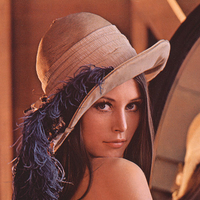
\includegraphics[scale=1]{img/convert_RGB.jpg}}}$
	$\vcenter{\hbox{\LARGE$\xrightleftharpoons[\text{YUVtoRGB}]{\text{RGBtoYUV}}$}}$
	$\vcenter{\hbox{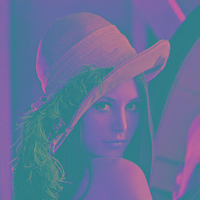
\includegraphics[scale=1]{img/convert_YUV.jpg}}}$
\end{figure}


\subsection{Implementación}

La solución implica recorrer la imagen completa aplicando la transformación a cada pixel de manera individual.

La implementación en C es relativamente trivial: se aplica la transformación correspondiente a cada componente de manera individual. En el caso de la transformación YUV a RGB existen algunos valores que podemos reutilizar, pero los demás cálculos se realizan como se indica en el problema.

Para la implementación en ASM definimos un par de constantes. La idea es que cada una represente una fila de la matriz de transformación. De esta manera, podemos calcular los 3 componentes fuente de cada componente destino en simultaneo.

Para los siguientes ejemplos se utiliza el filtro RGB2YUV, pero la implementación del filtro inverso es muy similar.

Primero, se definen 3 máscaras. Cada una se utilizará para crear una de las componentes finales:

\begin{center}
	\xmm{9} \xmmDoubleWordSmall{66}{129}{25}{0}

	\xmm{10} \xmmDoubleWordSmall{-38}{-74}{112}{0}

	\xmm{11} \xmmDoubleWordSmall{112}{-94}{-18}{0}
\end{center}

Para cada pixel, desempaquetamos sus componentes a tamaño doubleword. Esto es porque los valores que multiplicamos y sumamos pueden exceder el límite de una word, y perderíamos precisión o retornaríamos valores inválidos.

Cada pixel es copiado 3 veces, una por componente destino (en este caso, Y, U y V):

\begin{center}

	\xmm{1} \xmmDoubleWordSmall{R}{G}{B}{0}

	\xmm{14} $\leftarrow$ \xmm{1}

	\xmm{15} $\leftarrow$ \xmm{1}

\end{center}

Luego, se multiplican estas copias del pixel por la máscara correspondiente:

\begin{center}

	\texttt{PMULLD} \xmm{14}, \xmm{9} \hfill

	\xmm{14} \xmmDoubleWordSmall{$Y'_R$}{$Y'_G$}{$Y'_B$}{0}

	\texttt{PMULLD} \xmm{15}, \xmm{10} \hfill

	\xmm{15} \xmmDoubleWordSmall{$U'_R$}{$U'_G$}{$U'_B$}{0}

	\texttt{PMULLD} \xmm{1}, \xmm{11} \hfill

	\xmm{1} \xmmDoubleWordSmall{$V'_R$}{$V'_G$}{$V'_B$}{0}
	
\end{center}

Por último, estos valores intermedios se suman horizontalmente para crear las componentes finales:

\begin{center}

	\texttt{PHADDD} \xmm{15}, \xmm{14} \hfill

	\xmm{15} \xmmDoubleWordSmall{$Y'_{R+G}$}{$Y'_B$}{$U'_{R+G}$}{$U'_B$}

	\texttt{PHADDD} \xmm{1}, \xmm{1} \hfill

	\xmm{1} \xmmDoubleWordSmall{$V'_{R+G}$}{$V'_B$}{$V'_{R+G}$}{$V'_B$}

	\texttt{PHADDD} \xmm{1}, \xmm{15} \hfill

	\xmm{1} \xmmDoubleWordSmall{$Y'$}{$U'$}{$V'$}{$V'$}

\end{center}

Como se puede ver, al sumar se genera un valor duplicado al final. El mismo se genera porque las imagenes tienen 3 componentes y \texttt{PHADDD} toma siempre 2 parámetros. Esto no afecta la correción del filtro, ya que no estamos trabajando con el componente alfa y el mismo puede ser descartado.

Por último, estos componentes se denotan con $'$ porqe los mismos no son los valores finales: debemos aplicar 2 sumas y un shift a todos los componentes para finalizar la conversión. Para las sumas utilizamos nuevamente constantes precargadas en un registro XMM.

Ya que contamos con registros de 128 bits y cada pixel mide 32 bits de ancho (RGBA), podemos cargar 4 pixeles de la memoria por iteración. Los mismos son empaquetados y desempaquetados, y la lógica se encuentra cuadruplicada para procesar todos. Esto se hace para reducir el impacto de los accesos a memoria y los saltos condicionales.

Un detalle importante que aplica a este filtro es la independencia entre todos los pixeles, y la independencia de los mismos con respecto a su posición. Este detalle nos permite recorrer la imagen no como una matriz de pixeles sino como una lista continua de tamaño $w \times h$.


\subsection{Análisis preeliminar}
\subsubsection*{Comparación de rendimiento de ASM vs C}

Para realizar un análisis preliminar del rendimiento de los algoritmos, debimos medir los tiempos de ejecución de los mismos. Por claridad, unificamos el criterio utilizados para las mediciones a lo largo de todo el trabajo práctico. Los detalles de dicho critero se encuentran en el apéndice correspondiente.

Como ambos filtros son muy similares, los podemos comparar lado a lado:

\begin{center}
	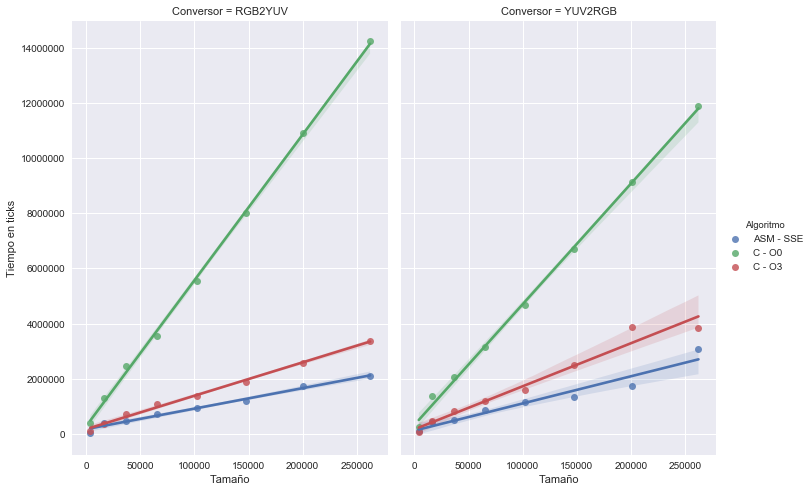
\includegraphics[scale=0.5]{img/conversores_CvsASMvsO3.png}
\end{center}

Por un lado, se puede notar una diferencia enorme en la performance del algoritmo escrito en C contra el escrito en ASM. Al compilar con optimizaciones, la brecha de performance baja drásticamente. Sospechamos que esto se debe a un uso más exhaustivo de los registros en lugar de acceder constantemente a memoria. Sin embargo, se puede ver que el algoritmo escrito con instrucciones SIMD sigue siendo más óptimo (hasta casi 60\% del tiempo, 2090676 en ASM vs 3377772 en C con \texttt{-O3}). Si bien la diferencia es visiblemente menor, y nuestras mediciones contaron con un poco de ruido, la diferencia porcentual es visible y relevante.

Por otro lado, se puede ver que en O0 el conversor YUV a RGB performa mejor que su contraparte RGB a YUV (con una diferencia de más de 10\%). Esto posiblemente se deba a ciertas operaciones que como mencionamos se repiten, y por ende podemos pre-calcular y reutilizar valores intermedios.

\subsection{Experimentación}

A modo de experimentación, decidimos probar con distintas imágenes con distintas proporciones. Los aspectos generales de la experimentación se encuentran detallado en los apéndices.

\begin{center}
	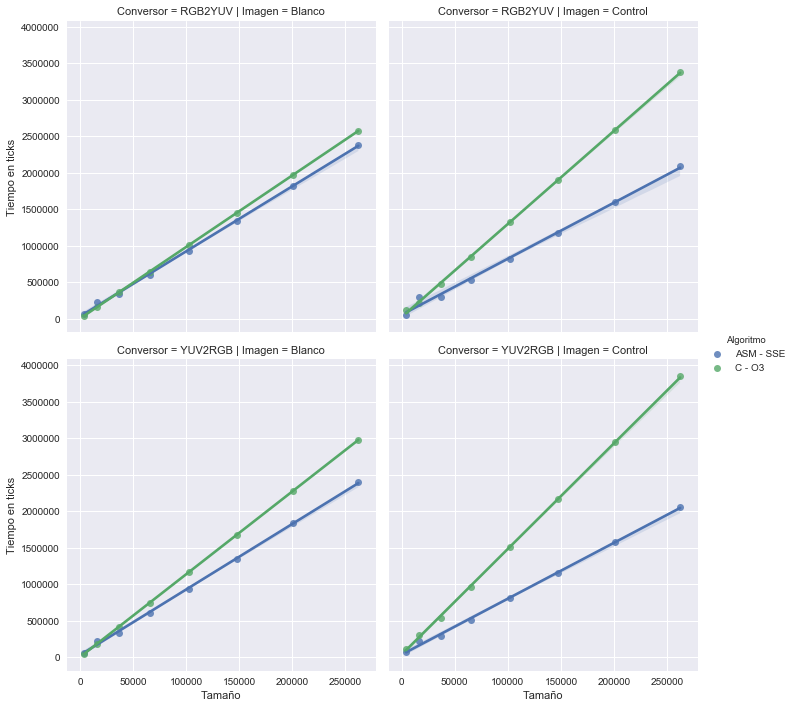
\includegraphics[scale=0.5]{img/conversores_blanco.png}
\end{center}

De cara a la experimentación, esperábamos que los algoritmos fuesen agnósticos a la mayoría de los detalles de la entrada. Sin embargo, al probar utilizando un bitmap blanco, podemos ver que la saturación de las componentes tiene un efecto visible en el tiempo de ejecución de los filtros. No solo eso, el bitmap afecta de manera positiva a la implementación en C, mientras que impacta de forma negativa a su contraparte SSE.

Nuestra teoría frente a esto es que la saturación puede ser optimizada en el caso de C (se pueden evitar algunos cálculos si se ve que el resultado estará saturado). Por otro lado, en ASM el procesador detecta que los componentes generan overflow y debe realizar el ajuste necesario para conservar un valor válido y saturado.